%----------------------------------------------------------------------------
\chapter{Presentation layer}

\section{Low level graphical challenges}

By using near-machine graphical interfaces, we lose certain simplified operations, for instance the ability to draw complex three-dimensional shapes directly from code. Most graphics cards have certain predispositions about the data they process, and in low-level cases, our program can't guarantee that those rules will be followed. LibGDX provides strong foundations in place of ready-made solutions, which the developer can use to implement or in some cases, disregard the GPU's written or unwritten requests. These include the following examples.
% A gépközeli grafikai interfészek használatával elveszítünk bizonyos egyszerűsített műveleteket, például a komplex alakzatok kódból történő közvetlen felrajzolását. A legtöbb grafikus kártya bizonyos feltételezésekkel él a rajta átfutó adatok feldolgozásakor, és így ezek teljesülésére sem képes garanciát vállalni a programunk. A libGDX kész megoldások helyett erős alapokat biztosít, amivel a fejlesztő saját döntése szerint implementálhatja vagy eseti alapon figyelmen kívül hagyhatja a GPU írott-íratlan igényeit; pár példát bemutatok ezekből.

\subsection{Triangulation, ear-clipping algorithm}

Triangles are the most commonly used basic two-dimensional shape that is supported without too many caveats on all platforms. Therefore, it's advisable to reduce any displayed models to a group of them.
%A két dimenziós háromszög a leggyakoribb elemi alakzat, amit minden platform grafikus interfésze feltétel nélkül támogat; célszerű lenne tehát a modelleket ezek összességére redukálni.

One geometrically intuitive division operation is the ear-clipping algorithm. An ear is defined as a triangle made up of three successive vertices of a polygon, where the middle vertex is convex -- in that point, the shape's inner angle must not exceed 180 degrees ($\pi$ raidans).\cite{TriangulationByEarClipping} Areas defined by such triples are guaranteed to be subtractable from the polygon's area, since by definition, they can not contain any holes, removing the need to compensate for empty space. The action can then be repeated on the remaining area, each successive step will result in a new triangular piece; when only three vertices remain, we have achieved our goal of subdivision.
% Geometriailag intuitív felosztó eljárás a fülvágó algoritmus (ear-clipping algorithm). Fül alatt olyan háromszöget értünk, amit egy poligon egymást követő három csúcspontja alkot, melyek közül a középső konvex -- tehát az adott pontban a sokszög belső szöge legfeljebb 180 fok ($\pi$ radián).\cite{TriangulationByEarClipping} Az ilyen hármasok által határolt terület garantáltan kivonható a poligonéból, mivel definíció szerint nem lehet lyuk vagy kihagyás benne, így nem kell kompenzálni az üres térért. Az eljárás a megmaradt területre megismételhető, és minden lépés egy újabb háromszög alakú részletet fog eredményezni; így a célunkat el is érjük, amikor már mindössze három csúcspont marad.

The goal of this algorithm is to create a list of vertex indices that should be connected into triangles, in order to cover the original polygon fully and efficiently. As a useful side effect, this makes calculating the mathematical area trivial as well.
% Az algoritmus célja tehát a fent leírt módszerrel kiszámítani, hogy egy tetszőleges sokszög lefedéséhez milyen módon kell háromszögekké összekötni a kapott vertexeket. Hasznos mellékhatás, hogy ezzel a sokszög területének összegzése is triviálissá válik.

In the case of libGDX, the EarClippingTriangulator class takes care of this common use case. Following OpenGL idioms, the relevant function requests floating point values (vectors decomposed into their axes), and it results in a list of whole number indices -- every group of three defines a triangle to be created.
%A libGDX esetében a gyakran visszatérő felhasználásnak köszönhetően külön osztály gondoskodik erről (EarClippingTriangulator). Az OpenGL idiómáinak megfelelően lebegőpontos értékekre bontott vektorokat kér bemenetként, eredménye pedig egy egyszerű, indexekből álló lista -- ennek elemei hármasával határoznak meg egy háromszöget.

\begin{lstlisting}[caption=Example usage of the EarClippingTriangulator class]
    val floats = baseNodes.flatMap { listOf(it.x, it.z) }.toFloatArray()
    val triangles: ShortArray
    val triangulator = EarClippingTriangulator()
    triangles = triangulator.computeTriangles(floats)
\end{lstlisting}

\subsection{Winding order}

Many graphical effects - including lighting - require knowledge of the affected faces' normal vectors. In the mathematical sense, this means a direction which is perpendicular to the whole surface, when applied to any contained point of it. %TODO meh 
When observing the side from this particular direction (the vector between the camera and a given point of the face can be represented as a multiple of the normal), the apparent size is at its largest -- in layman's terms, we're seeing the front without any rotations around axes that don't match the normal.% Számos effektus, például megvilágítás alkalmazásához szükséges ismerni az érintett lapok normálvektorát. Matematikai értelemben ez olyan irányt jelent, ami egy felület tetszőleges pontjában merőleges a teljes felületre. Ebből az irányból nézve a felület látszólagos mérete a lehető legnagyobb, mivel köznyelvileg "szemből" látjuk a sokszöget, egyik irányba sincs elforgatva.

The visibility of a polygon can technically also be treated as an effect. To reduce the number of draw calls, it's advisable to only handle faces that have their intended front side visible from the camera's perspective. By default, OpenGL utilises "back-face culling": the spectator can only see shapes where the order of vertices is counter-clockwise (when plotted in relation to the vector connecting the viewpoint and the weighted center of the polygon). This behaviour is modifiable as follows.
%Grafikai hatásnak tekinthető az is, hogy egyáltalán látható-e egy poligon. A kirajzolási műveletek számának csökkentése miatt célszerű csak azokat a lapokat számba venni, amiknek a kívánt oldala mutat a kamera felé. Az OpenGL alapértelmezetten "back-face culling" elven működik: a néző csak azokat az alakzatokat látja, amiknek a nézőpontot és az alakzat középpontját összekötő vektor körüli vertex-sorrendje az óramutató járásával ellentétes. Ez a viselkedés az alábbiak szerint módosítható.

\begin{lstlisting}[caption=Example for changing OpenGL's culling properties through libGDX]
    Gdx.gl.glEnable(GL40.GL_CULL_FACE) //enabling
    Gdx.gl.glCullFace(GL40.GL_BACK) //setting filtered side (rear)
    Gdx.gl.glFront(GL40.CW) //changing the intended winding order to clockwise
\end{lstlisting}

\subsection{Using the main thread}

In contrast to the project's simulation module, the user interface is difficult to parallelise. OpenGL functions are usually not thread-safe, requesting and modifying a single graphical context from multiple areas of code is dangerous and will often lead to crashes.

%A projekt szimulációs részével szemben a megjelenítés nehezen párhuzamosítható. Az OpenGL műveletek általában nem szálbiztosak, egy grafikai kontextust egy időben több helyről használni és módosítani nem érdemes; programunk futása hamar hibára fut.

The graphics library abstracts communication with the operating system and GPU as much as possible. In return it's the developer's responsibility to reduce GPU calls to the absolutely necessary amount. While unique calls are being processed, the GPU can't pass newly created frames to the processor, which is visible as the screen 'freezing' -- this is easily observable in the chapter dedicated to performance. 

%A grafikus könyvtár a lehető legjobban elrejti az operációs rendszerrel és GPU-val történő kommunikációt, cserébe viszont a fejlesztőnek ügyelnie kell arra, hogy az abszolút szükséges mennyiségre csökkentse a GPU hívásokat. Amíg egyedi kérések feldolgozása történik, a kártya nem tud újabb képkockákat átadni a processzornak, a monitoron tehát "megfagy" az animáció -- ez a későbbi, teljesítményt taglaló fejezetben jól látható.

Aside from frame construction, the program only uses the main graphical thread for creating unique models for each building, as this can't reasonably be done on the CPU. I decided against a complex thread-scheduling solution, as the GPU  only receives a heavy workload when creating a new save, or loading an OSM buffer file. When programming, I only had to built on available tools; I used a simple lambda function to obtain the main thread context when needed.

%A programban a fő szálat egyetlen helyen használom jelentősen a képalkotást leszámítva. A vonalakkal meghatározott épületek egyedi modelljét csak a GPU képes legyártani. A végső szoftverben a szálhasználat ütemezése helyett szokásosnak mondható módon betöltő-képernyő jelenik meg új mentés vagy adatcsomag előkészítése közben. Programozási szempontból csupán a meglévő eszköztárra kellett építenem, lambda függvényt készítettem a fő szál kontextusának tetszőleges szálon történő megszerzéséhez.

\begin{lstlisting}[caption=Helper function for getting the draw thread]
private suspend fun <T> runOnRenderThread(block: () -> T): T {
        return suspendCoroutine { continuation ->
            Gdx.app.postRunnable {
                continuation.resume(block())
            }
        }
    }
\end{lstlisting}

\section{Implementation}
The program's visual part can be divided into modules. Aside from the interactive, three-dimensional OpenGL scene showcasing the buildings, there exist multiple independent components, aiding user communication.

%A program grafikus része modulokra bontható. Az épületek bemutatására hivatott interaktív, három dimenziós OpenGL teret csomagoló, főszerepű jeleneten kívül több független, felhasználói kommunikációt megvalósító komponens is létezik.

\section{The main scene}
Buildings are presented in a simplified manner, ignoring any vertical terrain changes. Stylistically, it was inspired by contemporary city building video games (such as SimCity and Cities: Skylines), as well Google Earth.

%A grafikus felület egyszerűsített, domborzatot figyelmen kívül hagyó módon ábrázolja az egyes épületeket. Stílusa inspirációt merít a kortárs városépítő videojátékok (SimCity, Cities: Skylines) és a Google Earth kinézetéből. %TODO: felülnézet?
\begin{figure}[!ht]
    \centering
    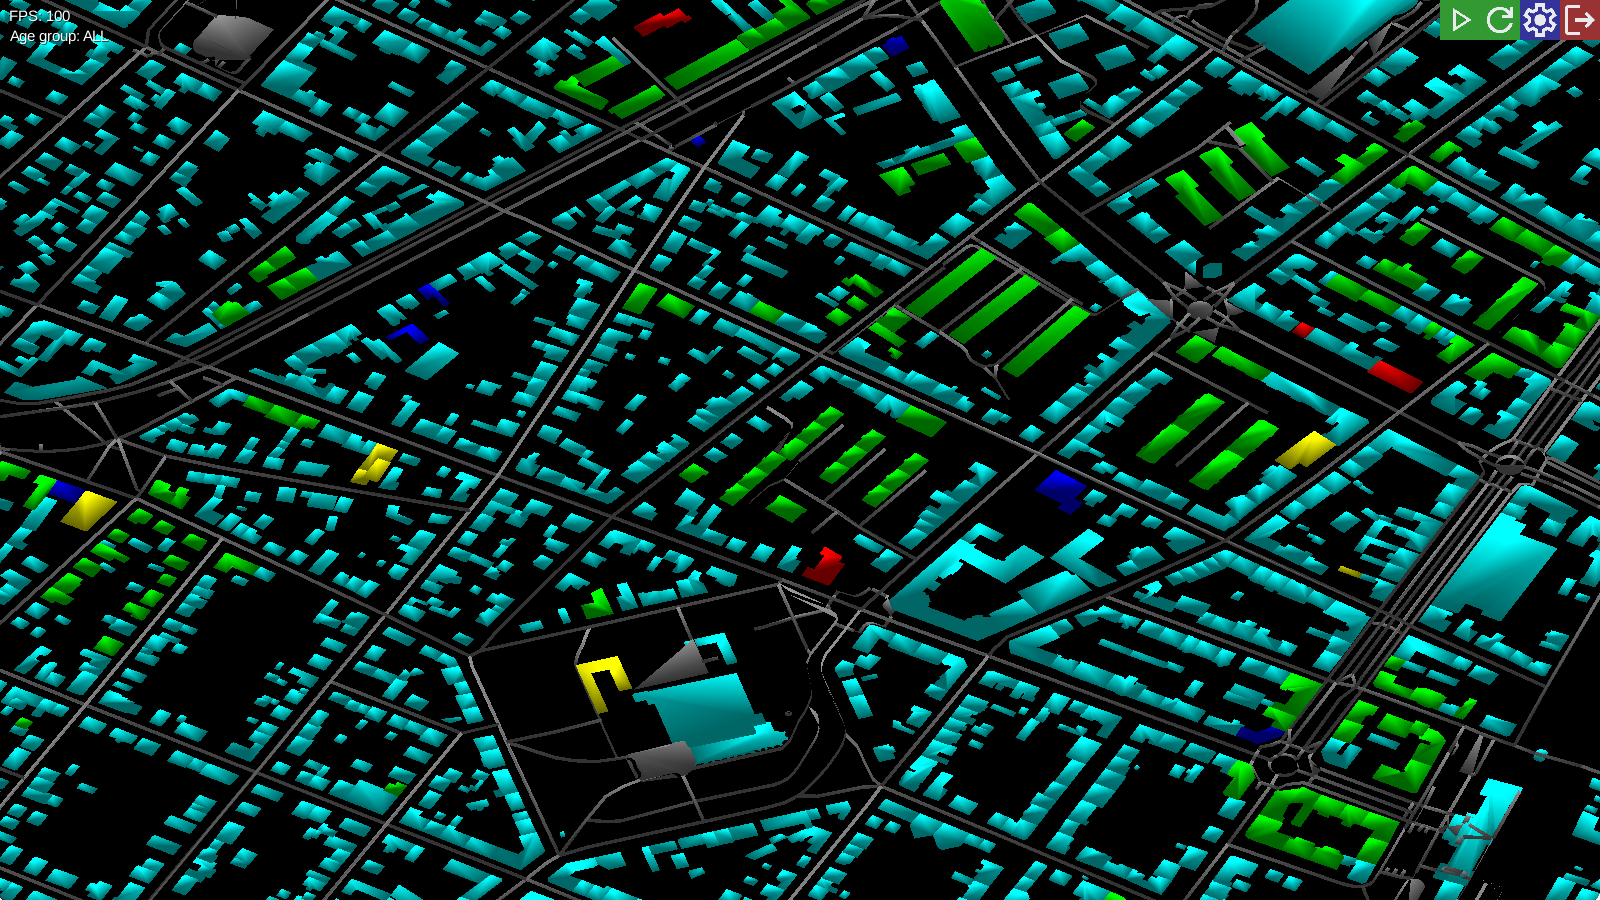
\includegraphics[width=150mm, keepaspectratio]{images/main_graphics_view.png}
    \caption{The main page of the app, with a "false 3D" view}
\end{figure}

\subsection{Custom camera control}

A libGDX jelenetei egyetlen bemenetet feldolgozó adapter objektumot, vagy azok összességéből készült multiplexert képesek tárolni. A könyvtár készítői által ajánlott alapértelmezett 3D keretprogram\cite{basic3DlibGDX} a CameraInputController osztályt használja; ez az eseménykezelő az egérrel végzett forgatást és nagyítást adja hozzá az azt meghívó jelenetnek.
A publikus InputAdapter interfészre támaszkodva saját kamera- illetve menüfunkciókat fejlesztettem. A megtekintési szög zárolva van, a felhasználó rögzített felülnézetből vizsgálhatja a backend adataiból készült képet. A mozgatás kihasználja a kamera képkockánként szükséges frissítését. A navigációs gombok megnyomása bizonyos mennyiséget hozzáad a jelenlegi a célmozgáshoz, és ez a mérőszám képkockánként százalékosan csökken, ahogy a kamera halad. A számláló kellően kicsi értéke mellett a mozgás azonnal befejeződik.
Ennek eredménye egy jól kinéző sebességkezelés, ami elkerüli a robotikus, hirtelen irányváltozásokat. Mivel egyszerre több parancs végrehajtása is történhet, minden, a kamera állapotát változtató függvény mutex\footnote{mutual exclusivity} zár alá esik; enélkül a képkockák kirajzolása közben ütköző lépések a képernyő ugrálását idéznék elő.
% TODO code section

\
 Egy komplexum, de akár az azt határoló vonalak által leírt poligon is lehet konkáv, így a teljes modellek felépítéséhez a fülvágó algoritmust használtam.

A backend-ről származó adatokból természetesen nem csak az entitások pozíciója, formája lényeges, az OpenStreetMap adathalmaz alapján csoportosíthatók és színezhetők  
